\chapter{Фазор}
\label{ch:intro}

Фазор (от англ. phasor) — это комплексное число, которое описывает амплитуду и фазу гармонического сигнала при фиксированной частоте. \\

\begin{figure}[ht]
    \centering
    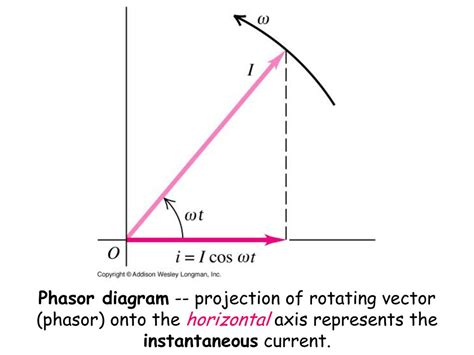
\includegraphics[width=1.0\textwidth]{Phasor.png}
    \caption{Геометрическая интерпретация фазора}
\end{figure}

Комплексное гармоническое колебание можно представить в виде

\[
A e^{i(\omega_0 t + \varphi)} = A\big(\cos(\omega_0 t + \varphi) + i\sin(\omega_0 t + \varphi)\big).
\]

Используя тригонометрические тождества Эйлера

\begin{figure}[ht]
    \centering
    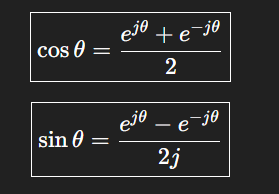
\includegraphics[width=1.0\textwidth]{euler_form.png}
    \caption{Тригонометрические тождества Эйлера}
\end{figure}

получим

\[
A \frac{e^{i(\omega_0 t + \varphi)} + e^{-i(\omega_0 t + \varphi)}}{2}
= \frac{A e^{i\varphi}}{2}\big(e^{i\omega_0 t} + e^{-i\omega_0 t}\big).
\]

Коэффициент \(A e^{i\varphi}\) и есть фазор.\\

3D визуализация фазора:

\begin{figure}[ht]
    \centering
    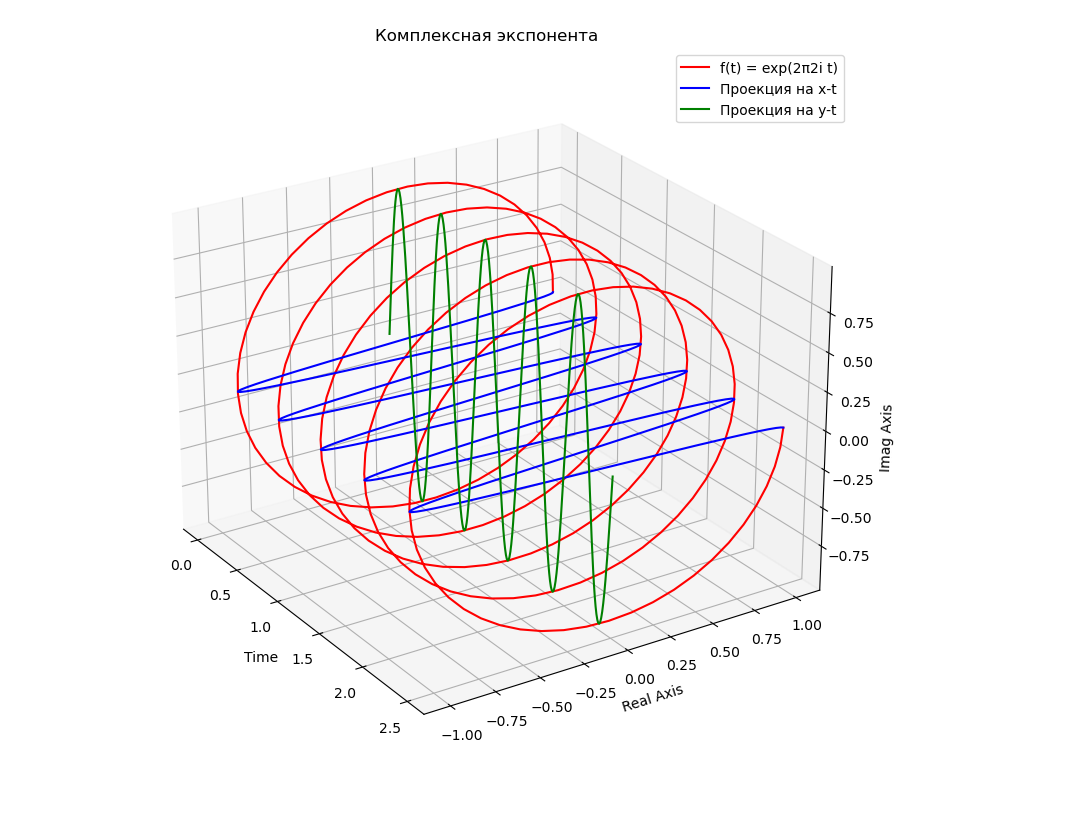
\includegraphics[width=1.0\textwidth]{phasor_vis.png}
    \caption{Пример фазора в трехмерном пространстве}
\end{figure}

\endinput